%%
%% Beginning of file 'sample.tex'
%%
%% Modified 2005 December 5
%%
%% This is a sample manuscript marked up using the
%% AASTeX v5.x LaTeX 2e macros.

%% The first piece of markup in an AASTeX v5.x document
%% is the \documentclass command. LaTeX will ignore
%% any data that comes before this command.

%% The command below calls the preprint style
%% which will produce a one-column, single-spaced document.
%% Examples of commands for other substyles follow. Use
%% whichever is most appropriate for your purposes.
%%
%\documentclass[12pt,preprint]{aastex}

%% manuscript produces a one-column, double-spaced document:

%\documentclass[manuscript]{aastex}
%\documentclass[onecolumn]{emulateapj}

%% preprint2 produces a double-column, single-spaced document:

 \documentclass[preprint2]{aastex}

%% Sometimes a paper's abstract is too long to fit on the
%% title page in preprint2 mode. When that is the case,
%% use the longabstract style option.

%% \documentclass[preprint2,longabstract]{aastex}

%% If you want to create your own macros, you can do so
%% using \newcommand. Your macros should appear before
%% the \begin{document} command.
%%
%% If you are submitting to a journal that translates manuscripts
%% into SGML, you need to follow certain guidelines when preparing
%% your macros. See the AASTeX v5.x Author Guide
%% for information.

\newcommand{\vdag}{(v)^\dagger}
\newcommand{\myemail}{jbyrne@ifa.hawaii.edu}

%%I'm adding these -JPB
%\newcommand{\solphys}{{\it Solar Physics}}
%\newcommand{\aap}{    {\it Astronomy \& Astrophysics}}
%\newcommand{\aaps}{   {\it Astronomy \& Astrophysics Supplemental}}
%\newcommand{\apj}{    {\it Astrophysical Journal}}
%\newcommand{\apjl}{    {\it Astrophysical Journal Letters}}
%\newcommand{\jgr}{    {\it Journal of Geophysical Research}}
%\newcommand{\aapr}{    {\it Astronomy \& Astrophysics Review}}
%\newcommand{\grl}{    {\it Geophysical Research Letters}}
\newcommand{\lrsp}{    {\it Living Rev. Solar Phys.}}

\newcommand{\RNum}[1]{\uppercase\expandafter{\romannumeral #1\relax}}

\usepackage{subfigure}

%\makeatletter
%\newcommand*{\rom}[1]{\expandafter\@slowromancap\romannumeral #1@}
%\makeatother

%% You can insert a short comment on the title page using the command below.

%\slugcomment{Paper \RNum{2} of \RNum{2}}

%% If you wish, you may supply running head information, although
%% this information may be modified by the editorial offices.
%% The left head contains a list of authors,
%% usually a maximum of three (otherwise use et al.).  The right
%% head is a modified title of up to roughly 44 characters.
%% Running heads will not print in the manuscript style.

\shorttitle{Kinematics and Morphology of CMEs using CORIMP}
\shortauthors{Byrne et al.}

%% This is the end of the preamble.  Indicate the beginning of the
%% paper itself with \begin{document}.

\begin{document}

%% LaTeX will automatically break titles if they run longer than
%% one line. However, you may use \\ to force a line break if
%% you desire.

\title{Investigating the Kinematics and Morphology of Coronal Mass Ejections using the CORIMP Catalogue}

%% Use \author, \affil, and the \and command to format
%% author and affiliation information.
%% Note that \email has replaced the old \authoremail command
%% from AASTeX v4.0. You can use \email to mark an email address
%% anywhere in the paper, not just in the front matter.
%% As in the title, use \\ to force line breaks.

\author{Jason P. Byrne$^1$, Huw Morgan$^{1,2}$ and Shadia R. Habbal$^1$}
\affil{$^1$Institute for Astronomy, University of Hawai'i,\\2680 Woodlawn Drive, Honolulu, HI 96822, USA.}
\affil{$^2$Institute of Mathematics and Physics, Aberystwyth University,\\Ceredigion, Wales, SY23 3BZ.}
\email{jbyrne@ifa.hawaii.edu}

%% Notice that each of these authors has alternate affiliations, which
%% are identified by the \altaffilmark after each name.  Specify alternate
%% affiliation information with \altaffiltext, with one command per each
%% affiliation.


%% Mark off your abstract in the ``abstract'' environment. In the manuscript
%% style, abstract will output a Received/Accepted line after the
%% title and affiliation information. No date will appear since the author
%% does not have this information. The dates will be filled in by the
%% editorial office after submission.

\begin{abstract}

\end{abstract}


%% Keywords should appear after the \end{abstract} command. The uncommented
%% example has been keyed in ApJ style. See the instructions to authors
%% for the journal to which you are submitting your paper to determine
%% what keyword punctuation is appropriate.

\keywords{Sun: activity; Sun: corona; Sun: coronal mass ejections (CMEs)}

%% From the front matter, we move on to the body of the paper.
%% In the first two sections, notice the use of the natbib \citep
%% and \citet commands to identify citations.  The citations are
%% tied to the reference list via symbolic KEYs. The KEY corresponds
%% to the KEY in the \bibitem in the reference list below. We have
%% chosen the first three characters of the first author's name plus
%% the last two numeral of the year of publication as our KEY for
%% each reference.


%% Authors who wish to have the most important objects in their paper
%% linked in the electronic edition to a data center may do so by tagging
%% their objects with \objectname{} or \object{}.  Each macro takes the
%% object name as its required argument. The optional, square-bracket 
%% argument should be used in cases where the data center identification
%% differs from what is to be printed in the paper.  The text appearing 
%% in curly braces is what will appear in print in the published paper. 
%% If the object name is recognized by the data centers, it will be linked
%% in the electronic edition to the object data available at the data centers  
%%
%% Note that for sources with brackets in their names, e.g. [WEG2004] 14h-090,
%% the brackets must be escaped with backslashes when used in the first
%% square-bracket argument, for instance, \object[\[WEG2004\] 14h-090]{90}).
%%  Otherwise, LaTeX will issue an error. 

\section{Introduction}
\label{sect_intro}

\section{Numerical Differentiation Techniques (recap)}
When presented with a moving object through a sequence of image frames such that it is possible to measure its position at each time step, the technique of numerical differentiation is often used to derive the velocity and acceleration of the object. In the standard 2-point approach, it should be possible to derive the time evolution of a system at time step $t+\delta t$ according to the system values at time step $t$. This may be applied through the technique of forward, reverse or centre differencing, resulting in an estimate of the speed of the object at a specific time step given its positional information. More commonly, a 3-point Lagrangian interpolation is applied to better approximate the kinematics of a moving object by solving for the Lagrange polynomials that best fit across three given datapoints (e.g. \textsc{deriv.pro} in IDL). Each of these schemes is based upon the Taylor series expansion of a real function $f(t)$:
\begin{equation}
\label{taylor1}
f(t_0+\delta t) \; = \; f(t_0)+f'(t_0)\delta t +  \frac{f''(t_0)}{2!}(\delta t)^{2}  + ...
\end{equation}
but due to the approximation of an infinite series with a finite number of terms and iterations, an error must be associated with the result, based on its deviation from the true solution. Generally the Euler method is employed, using the formula:
\begin{equation}
y_{n+1} \; = \; y_n + h f(t_n, y_n)
\end{equation}
to solve the initial value problem $y'=f(t,y)$ given $y(t_0)=y_0$, where $h$ is the stepsize such that $t_n=t_0+nh$. The convergence of such an approximation to the actual solution is prone to two sources of error; truncation error (the difference between the true solution and the approximation) and round-off error (the limited precision of the approximation). Add to this fact that the data measurements themselves are subject to uncertainties in both the positional and temporal information, and the ability of the numerical differentiation techniques to derive kinematics becomes highly jeopardised, as shall be shown.

Given a function $x=f(u,\,v)$, the error propagation equation (based on the standard deviations $\sigma$ of the variables) is written:
\begin{equation}
\label{eqn_errorprop}
\sigma_x^2 \; = \; \sigma_u^2 \left(\frac{\partial x}{\partial u}\right) ^2 + \sigma_v^2 \left( \frac{\partial x}{\partial v} \right) ^2 + 2 \sigma_{uv}^2 \left( \frac{\partial x}{\partial u} \right) \left( \frac{\partial x}{\partial v} \right) + ...
\end{equation}
Specifically in the case of kinematic analyses, this is used to propagate the errors on the height-time data $r(t)$ into the velocity $v(t)$ and acceleration $a(t)$ profiles to determine the associated uncertainties. In the case of height-time data the covariance terms are zero because the quantities are uncorrelated.

In the case of relatively low sampling of the data, as in the case of coronagraph observations of CMEs, it is generally found that the simplest differentiation techniques are not applicable. The forward and/or reverse differencing techniques act to shift the kinematic profiles by one time-step, which is substantial enough to be of concern here (i.e., they derive a result at the current time-step, based on the pro-/preceeding time-step). Centre differencing employs the two neighbouring datapoints of the point under examination, and so is a better indication of the result at that time-step, but it fails at both endpoints. In any case these should not be employed when the spacing of the datapoints is unequal, i.e., when the cadence $\delta t$ is not constant, and so the 3-point Lagrangian interpolation technique is used for such cases (and gives the same result as the centre-difference otherwise, but includes the endpoints). The Lagrangian interpolation polynomial is given by:
\begin{eqnarray}
L(x) \; &=\; \sum_{j=0}^2 y_j l_j(x) \\ \quad \mbox{where} \quad
l_j(x) \; &=\; \prod_{i=0, i\neq j}^2 \frac{x-x_i}{x_j-x_i} 
\end{eqnarray}
The derivative at point $x$ is given by $L'=\partial_x L(x)$. So for the case of height-time data being used to derive velocity (and similarly for acceleration) the associated error is given by:
\begin{equation}
\sigma_{v_1}^2 \,=\, \frac{\sigma_{r(t_2)}^2+\sigma_{r(t_0)}^2}{(t_2-t_0)^2} + v^2 \left( \frac{\sigma_{t_2}^2+\sigma_{t_0}^2}{(t_2-t_0)^2} \right)
\label{vel_err}
\end{equation}
with the endpoint errors derived from a weighting of the pro-/preceeding three datapoints, and therefore larger.

Although the 3-point Lagrangian is mathematically sound, its application to CME data has proved problematic due to the limitations of the data. The main drawback is that the noise level across the few, low-cadence measurements, often belies the actual trends of the data such that the numerical derivations of velocity and acceleration become untrustworthy and even misleading. As an example of this, we simulate a height-time profile of a CME that propagates with a constant acceleration of 2~m~s$^{-2}$ and initial velocity 300~km~s$^{-1}$, and add random noise of various levels up to a maximum of $\sim$20\%. An errorbar on each datapoint is determined by its distance from the true height-time profile, to represent the worst best-case scenario wherein all measurements lie on the very edge of the known error. Various instances of datapoint scatters result in erroneous trends in the velocity and acceleration profiles - even with the proper error treatment ascribed by the 3-point Lagrangian interpolation technique. Two such cases are shown in in Figure~\ref{sim_vels_thesis} where completely opposing acceleration trends are revealed, indicating that the nature of the scatter in the samples is not satisfactorily reflected in the derived kinematics and associated errors. The worry here is that for CMEs undergoing non-constant acceleration, the resulting trends in the derived profiles may be completely intractable via these methods. One possible assurance has been that instead of trusting the endpoints, even given their larger errorbars, they be removed. Figure~\ref{sim_vels_thesis} would then show three datapoints for CME velocity and one for acceleration, that would in the left case go somewhat toward removing the biased trend and implying a constant acceleration, while in the right case it would remain inconclusive. So qualitatively this might achieve a more accurate result and avoid assigning erroneous trends, especially to fast CMEs for which there are few datapoints.

Beyond the interest certainly in the initial acceleration from the forces that drive a CME to erupt, there is a real physical motivation to resolve the subsequent low or zero acceleration as precisely as possible. This is important for determining whether the predominant forces acting are such that the CME is, in general, undergoing continued driving (internal) forces, or positive or negative drag (external) forces, or most assuredly some interplay of both. Any changes to its acceleration that result from different phases of dominating force, and where or why this occurs, are of great interest. Yet this all remains somewhat elusive given the limitations of current CME data, especially as \citet{2007ApJ...657.1117W} demonstrate that the errors in the acceleration values can be of the same order as the accelerations typically measured. 


We investigate the output of the recently developed CORIMP catalogue with new techniques (and stringent error analyses) for deriving CME kinematics.


\begin{figure*}[ht]
\centering
\subfigure{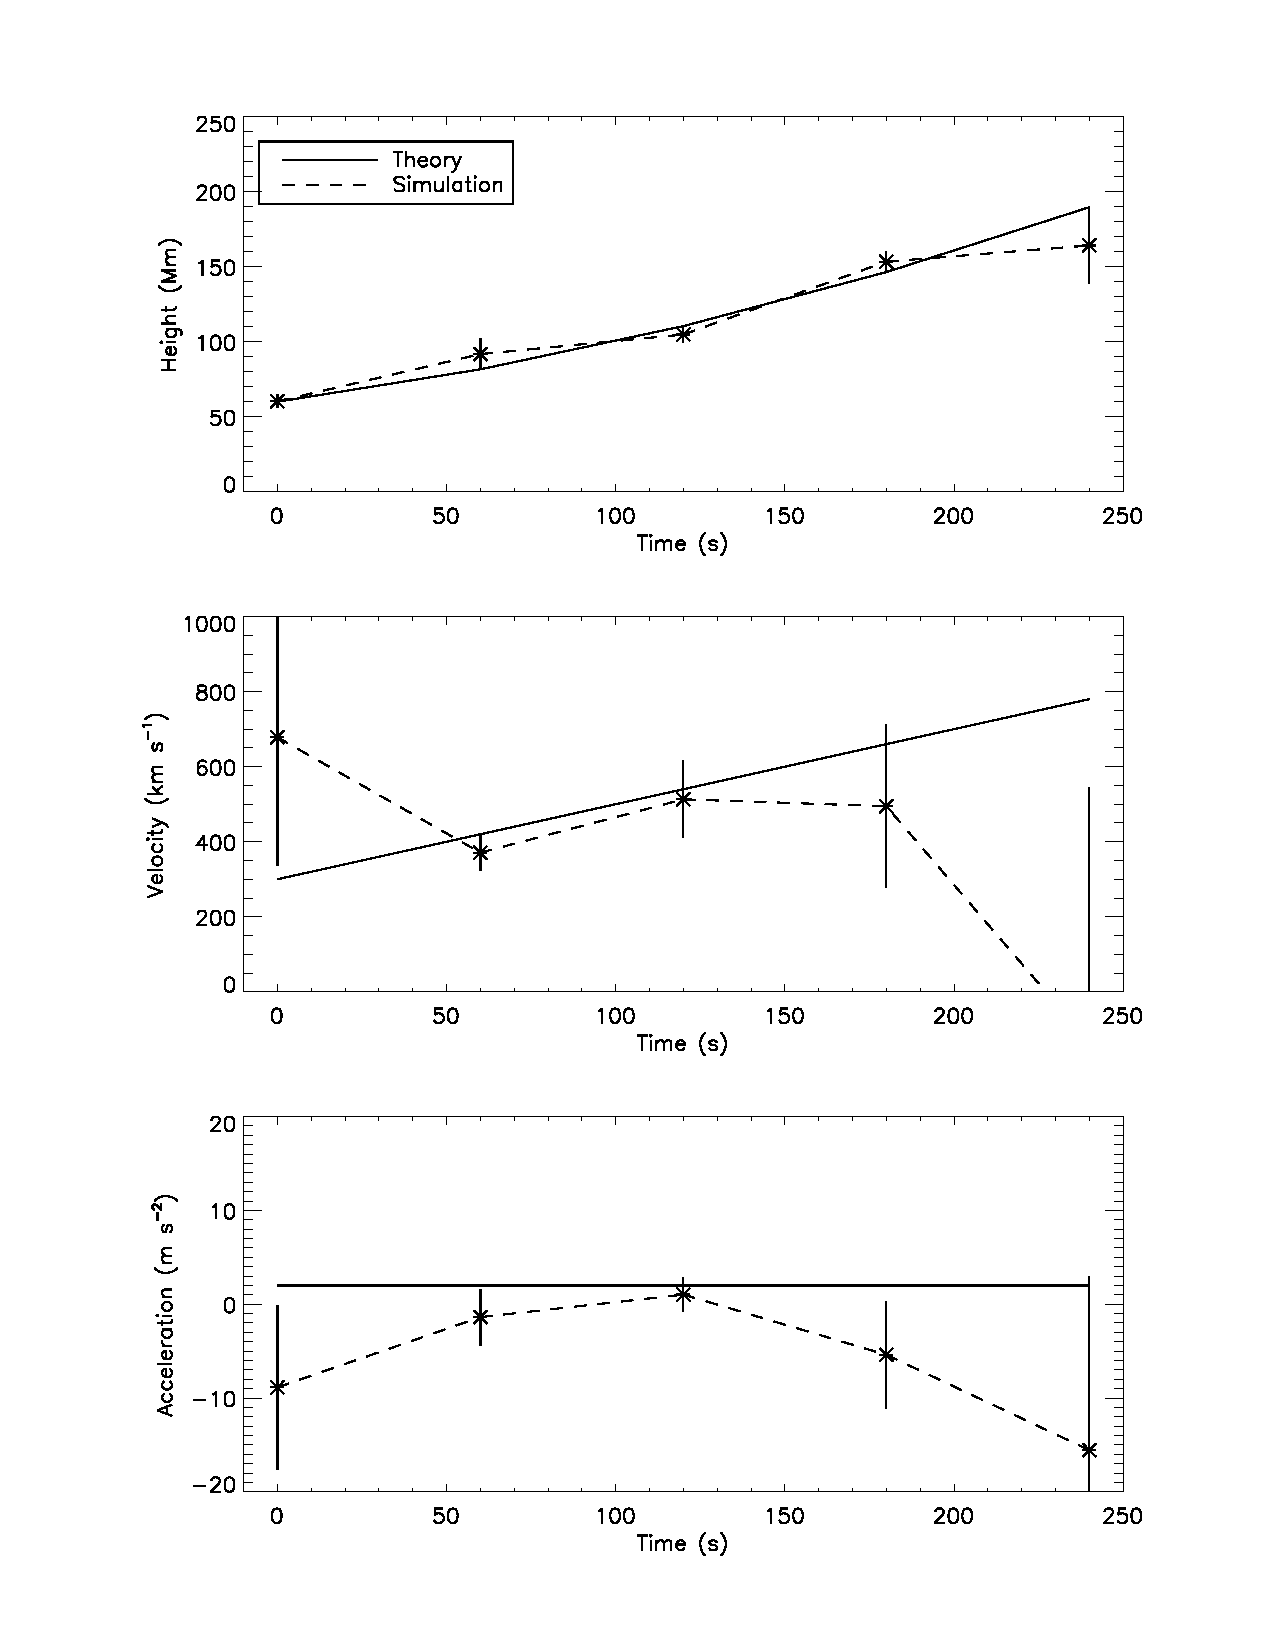
\includegraphics[scale=0.43, trim=110 50 70 70]{images/sim_vels_thesis1.pdf}}
\subfigure{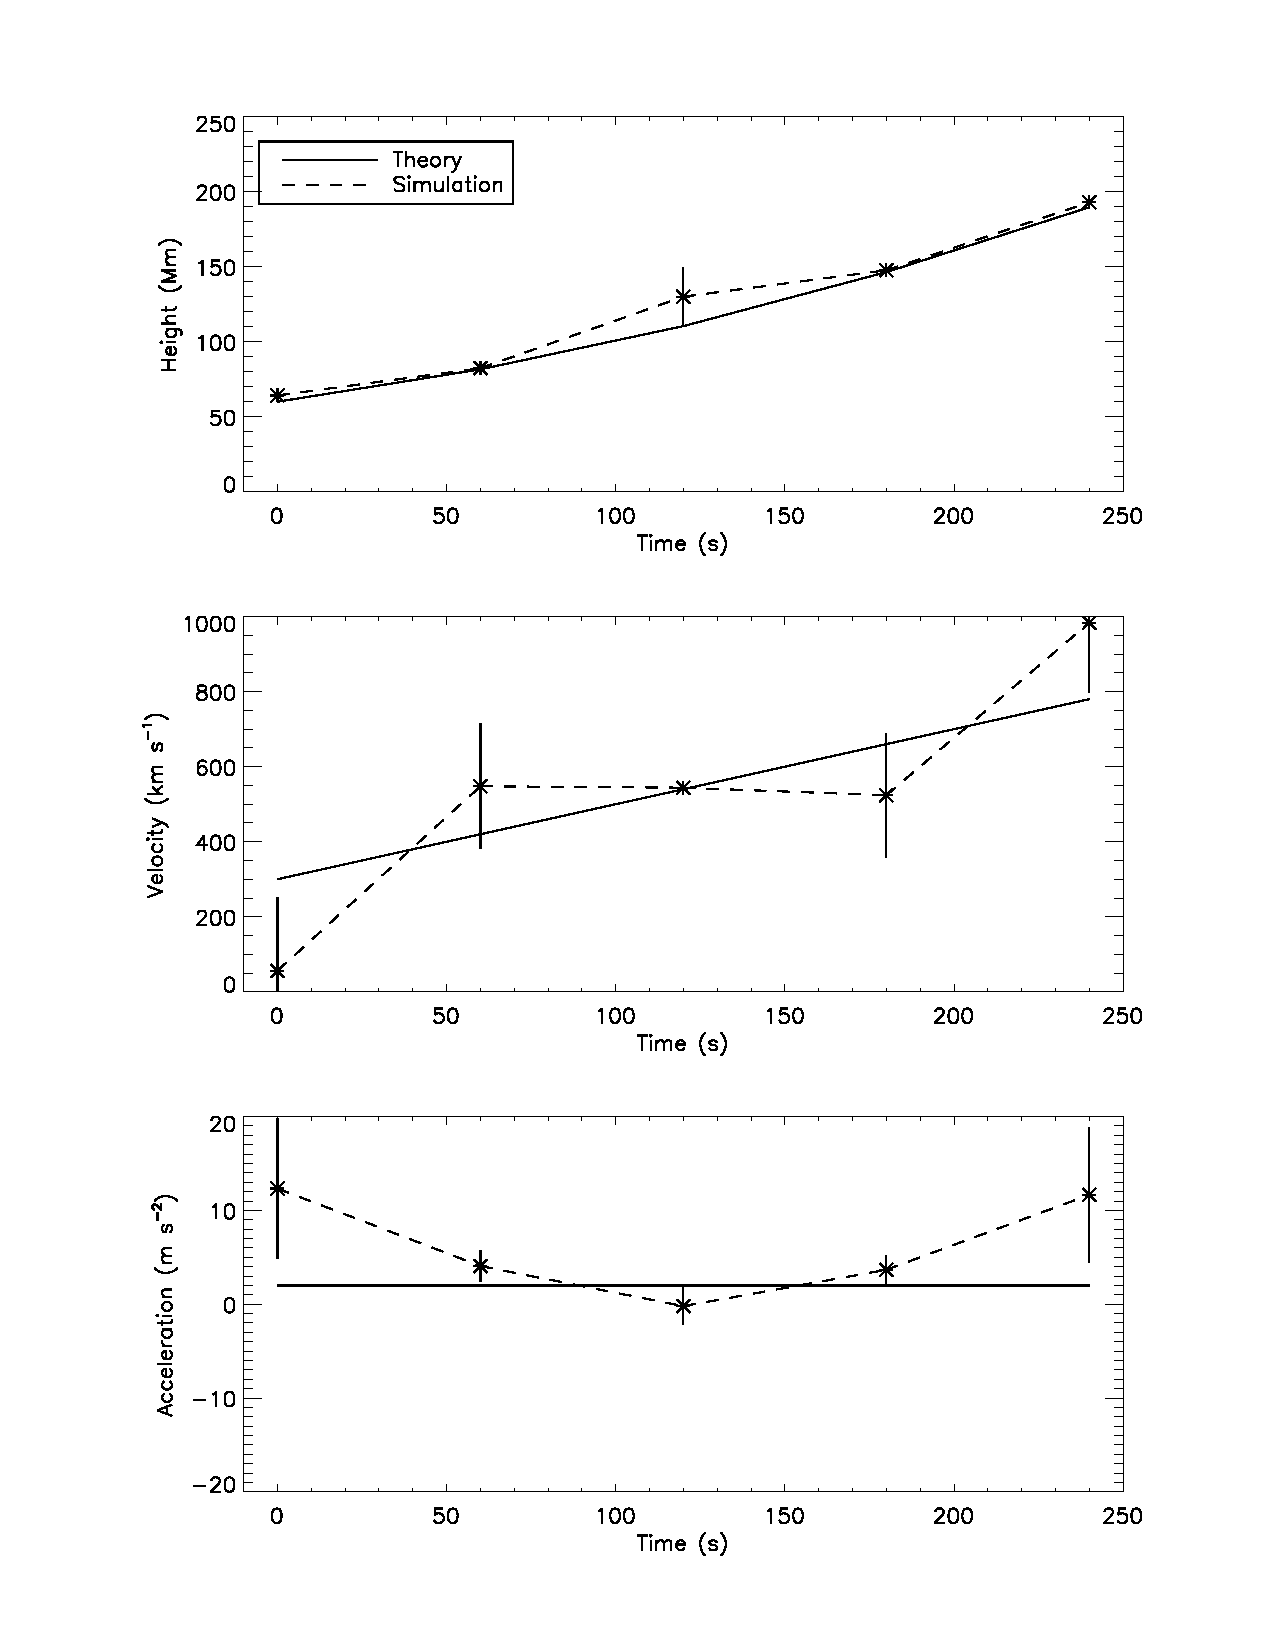
\includegraphics[scale=0.43, trim=70 50 110 70]{images/sim_vels_thesis2.pdf}}
\caption{A theoretical model for a CME with constant acceleration 2~m~s$^{-2}$ and initial velocity 300~km~s$^{-1}$, and two simulations of how the resulting profiles for a noisy sample of datapoints behave using 3-point Lagrangian interpolation.}
\label{sim_vels_thesis}
\end{figure*}


\section{Models}
\subsection{Testing for Constant Acceleration}




\subsection{Testing for Non-constant Acceleration}





\section{Conclusions}
\label{sect_conclusions}


%% If you wish to include an acknowledgments section in your paper,
%% separate it off from the body of the text using the \acknowledgments
%% command.

%% Included in this acknowledgments section are examples of the
%% AASTeX hypertext markup commands. Use \url without the optional [HREF]
%% argument when you want to print the url directly in the text. Otherwise,
%% use either \url or \anchor, with the HREF as the first argument and the
%% text to be printed in the second.

\acknowledgments

This work is supported by SHINE grant 0962716 and NASA grant NNX08AJ07G to the Institute for Astronomy. The SOHO/LASCO data used here are produced by a consortium of the Naval Research Laboratory (USA), Max-Planck-Institut fuer Aeronomie (Germany), Laboratoire d'Astronomie (France), and the University of Birmingham (UK). SOHO is a project of international cooperation between ESA and NASA. The STEREO/SECCHI project is an international consortium of the Naval Research Laboratory (USA), Lockheed Martin Solar and Astrophysics Lab (USA), NASA Goddard Space Flight Center (USA), Rutherford Appleton Laboratory (UK), University of Birmingham (UK), Max-Planck-Institut f\"{u}r Sonnen-systemforschung (Germany), Centre Spatial de Liege (Belgium), Institut d'Optique Th\'{e}orique et Appliqu\'{e}e (France), and Institut d'Astrophysique Spatiale (France). 

%% To help institutions obtain information on the effectiveness of their
%% telescopes, the AAS Journals has created a group of keywords for telescope
%% facilities. A common set of keywords will make these types of searches
%% significantly easier and more accurate. In addition, they will also be
%% useful in linking papers together which utilize the same telescopes
%% within the framework of the National Virtual Observatory.
%% See the AASTeX Web site at http://www.journals.uchicago.edu/AAS/AASTeX
%% for information on obtaining the facility keywords.

%% After the acknowledgments section, use the following syntax and the
%% \facility{} macro to list the keywords of facilities used in the research
%% for the paper.  Each keyword will be checked against the master list during
%% copy editing.  Individual instruments or configurations can be provided 
%% in parentheses, after the keyword, but they will not be verified.


%% Appendix material should be preceded with a single \appendix command.
%% There should be a \section command for each appendix. Mark appendix
%% subsections with the same markup you use in the main body of the paper.

%% Each Appendix (indicated with \section) will be lettered A, B, C, etc.
%% The equation counter will reset when it encounters the \appendix
%% command and will number appendix equations (A1), (A2), etc.


%% The reference list follows the main body and any appendices.
%% Use LaTeX's thebibliography environment to mark up your reference list.
%% Note \begin{thebibliography} is followed by an empty set of
%% curly braces.  If you forget this, LaTeX will generate the error
%% "Perhaps a missing \item?".
%%
%% thebibliography produces citations in the text using \bibitem-\cite
%% cross-referencing. Each reference is preceded by a
%% \bibitem command that defines in curly braces the KEY that corresponds
%% to the KEY in the \cite commands (see the first section above).
%% Make sure that you provide a unique KEY for every \bibitem or else the
%% paper will not LaTeX. The square brackets should contain
%% the citation text that LaTeX will insert in
%% place of the \cite commands.

%% We have used macros to produce journal name abbreviations.
%% AASTeX provides a number of these for the more frequently-cited journals.
%% See the Author Guide for a list of them.

%% Note that the style of the \bibitem labels (in []) is slightly
%% different from previous examples.  The natbib system solves a host
%% of citation expression problems, but it is necessary to clearly
%% delimit the year from the author name used in the citation.
%% See the natbib documentation for more details and options.

\bibliographystyle{apj.bst}
\bibliography{references.bib}  


%% Use the figure environment and \plotone or \plottwo to include
%% figures and captions in your electronic submission.
%% To embed the sample graphics in
%% the file, uncomment the \plotone, \plottwo, and
%% \includegraphics commands
%%
%% If you need a layout that cannot be achieved with \plotone or
%% \plottwo, you can invoke the graphicx package directly with the
%% \includegraphics command or use \plotfiddle. For more information,
%% please see the tutorial on "Using Electronic Art with AASTeX" in the
%% documentation section at the AASTeX Web site,
%% http://www.journals.uchicago.edu/AAS/AASTeX.
%%
%% The examples below also include sample markup for submission of
%% supplemental electronic materials. As always, be sure to check
%% the instructions to authors for the journal you are submitting to
%% for specific submissions guidelines as they vary from
%% journal to journal.

%% This example uses \plotone to include an EPS file scaled to
%% 80% of its natural size with \epsscale. Its caption
%% has been written to indicate that additional figure parts will be
%% available in the electronic journal.


%% Here we use \plottwo to present two versions of the same figure,
%% one in black and white for print the other in RGB color
%% for online presentation. Note that the caption indicates
%% that a color version of the figure will be available online.
%%


%% This figure uses \includegraphics to scale and rotate the still frame
%% for an mpeg animation.


%% If you are not including electonic art with your submission, you may
%% mark up your captions using the \figcaption command. See the
%% User Guide for details.
%%
%% No more than seven \figcaption commands are allowed per page,
%% so if you have more than seven captions, insert a \clearpage
%% after every seventh one.

%% Tables should be submitted one per page, so put a \clearpage before
%% each one.

%% Two options are available to the author for producing tables:  the
%% deluxetable environment provided by the AASTeX package or the LaTeX
%% table environment.  Use of deluxetable is preferred.
%%

%% Three table samples follow, two marked up in the deluxetable environment,
%% one marked up as a LaTeX table.

%% In this first example, note that the \tabletypesize{}
%% command has been used to reduce the font size of the table.
%% We also use the \rotate command to rotate the table to
%% landscape orientation since it is very wide even at the
%% reduced font size.
%%
%% Note also that the \label command needs to be placed
%% inside the \tablecaption.

%% This table also includes a table comment indicating that the full
%% version will be available in machine-readable format in the electronic
%% edition.


%% If the table is more than one page long, the width of the table can vary
%% from page to page when the default \tablewidth is used, as below.  The
%% individual table widths for each page will be written to the log file; a
%% maximum tablewidth for the table can be computed from these values.
%% The \tablewidth argument can then be reset and the file reprocessed, so
%% that the table is of uniform width throughout. Try getting the widths
%% from the log file and changing the \tablewidth parameter to see how
%% adjusting this value affects table formatting.

%% The \dataset{} macro has also been applied to a few of the objects to
%% show how many observations can be tagged in a table.


%% Tables may also be prepared as separate files. See the accompanying
%% sample file table.tex for an example of an external table file.
%% To include an external file in your main document, use the \input
%% command. Uncomment the line below to include table.tex in this
%% sample file. (Note that you will need to comment out the \documentclass,
%% \begin{document}, and \end{document} commands from table.tex if you want
%% to include it in this document.)

%% \input{table}

%% The following command ends your manuscript. LaTeX will ignore any text
%% that appears after it.

\end{document}

%%
%% End of file `sample.tex'.
